% =====================================================================
%  ch02b.tex ------ §2.2 共形场理论与 Jones 多项式（原书 p.63--p.75 上部）
%                 + §2.3 节标题与开头（原书 p.75 页末--p.76）
%  负责：tr06
% =====================================================================

% [原文 p.63]
% 注：跨块句「また，定理 2.3 を……拡張することもできる．」起于 p.62，按分工由 ch02a 写完；
%     本块从下一个句子「この場合は……」开始，不重复。
此时取 $\kappa=k+m$、$\eta=\exp(\pi\sqrt{-1}/m\kappa)$，同样的结果成立。

如命题 1.18 所述，共形块空间具有 Möbius 变换下的共变性。可知在 $V_{\lambda_1\cdots\lambda_n}$ 上不仅有辫群 $B_n$ 的作用，映射类群 $M_{0,n}$ 也线性地作用。这里 $M_{0,n}$ 是下述同痕类构成的群：从 Riemann 球面挖去以 $p_1,\dots,p_n$ 为中心的充分小圆盘所得的曲面到自身、固定边界且保持定向的微分同胚全体，按同痕分类。特别地，关于与以 $p_j$ 为中心的圆盘边界平行的曲线 $C_j$ 的 Dehn 扭转是标量映射 $\exp(-2\pi\sqrt{-1}\Delta_j)$。所谓 Dehn 扭转，指沿 $C_j$ 剪开、旋转 $2\pi$ 后粘回的微分同胚（参见 §2.4 图 2.24）。映射类群的作用将在 §2.4 重新讨论。

\section{共形场理论与 Jones 多项式}

\takeaway{利用 KZ 连接的和乐，即辫群在共形块空间上的作用，把带定向与 framing 的链环剖成基本 tangle 逐段合成线性映射，得到链环不变量；$q$ 取单位根时它给出 Jones 多项式的特殊值，并可推广为 tangle 算子。}

本章仍只处理 Lie 代数 $\fg$ 为 $sl_2(\C)$ 的情形。在 Riemann 球面上取 $n$ 个互不相同的点 $p_1,\dots,p_n$，其坐标为 $z_1,\dots,z_n$。固定称为 level 的正整数 $k$；对 level $k$ 的最高权组 $\bm{\lambda}=(\lambda_1,\dots,\lambda_n)$，§1.4 定义了共形块空间 $\cH(\bm{p},\bm{\lambda})$。进而 §1.5 证明：当点 $\bm{p}=(p_1,\dots,p_n)$ 变动时，共形块空间构成 Riemann 球面上 $n$ 个互异点的构形空间 $\Conf_n(\CP^1)$ 上的向量丛，其上自然有称为 KZ 连接的平坦联络。由该联络的和乐，得到辫群在共形块空间上的作用。

下面说明：利用上述辫群在共形块空间上的作用，可以构造链环的拓扑不变量。先说明关于链环的术语。链环（link）是把若干个互不相交的 $S^1$ 之并嵌入 $S^3$ 的嵌入
\[
  f: S^1\cup\cdots\cup S^1 \longrightarrow S^3
\]
每个 $S^1$ 的像称为链环的分支，并记 $L=L_1\cup\cdots\cup L_m$
% [原文 p.64]
来表示。特别地，只有一个分支的链环称为纽结（knot）。链环 $L,L'$ 等价，是指存在保持 $S^3$ 定向的同胚 $h$，使 $L'=h(L)$。对于每个分支都给定定向、且有两个分支 $L_1,L_2$ 的链环，其环绕数（linking number）$\operatorname{lk}(L_1,L_2)$ 是基本不变量。它定义为以 $L_1$ 为边界、$S^3$ 内带定向的曲面与 $L_2$ 的交点数。环绕数也可在链环 $L_1\cup L_2$ 的投影图中计算：取 $L_1$ 与 $L_2$ 的正交叉数减去负交叉数，再除以 $2$。这里正交叉、负交叉按图 2.7 定义。$L$ 的 framing（标架）是表示链环各分支法丛平凡化的整数，由链环分支与其管状邻域上闭曲线的环绕数给出。为表示 framing，有时也如图 2.7 那样把链环画成带状。

\begin{figure}[htbp]
  \centering
  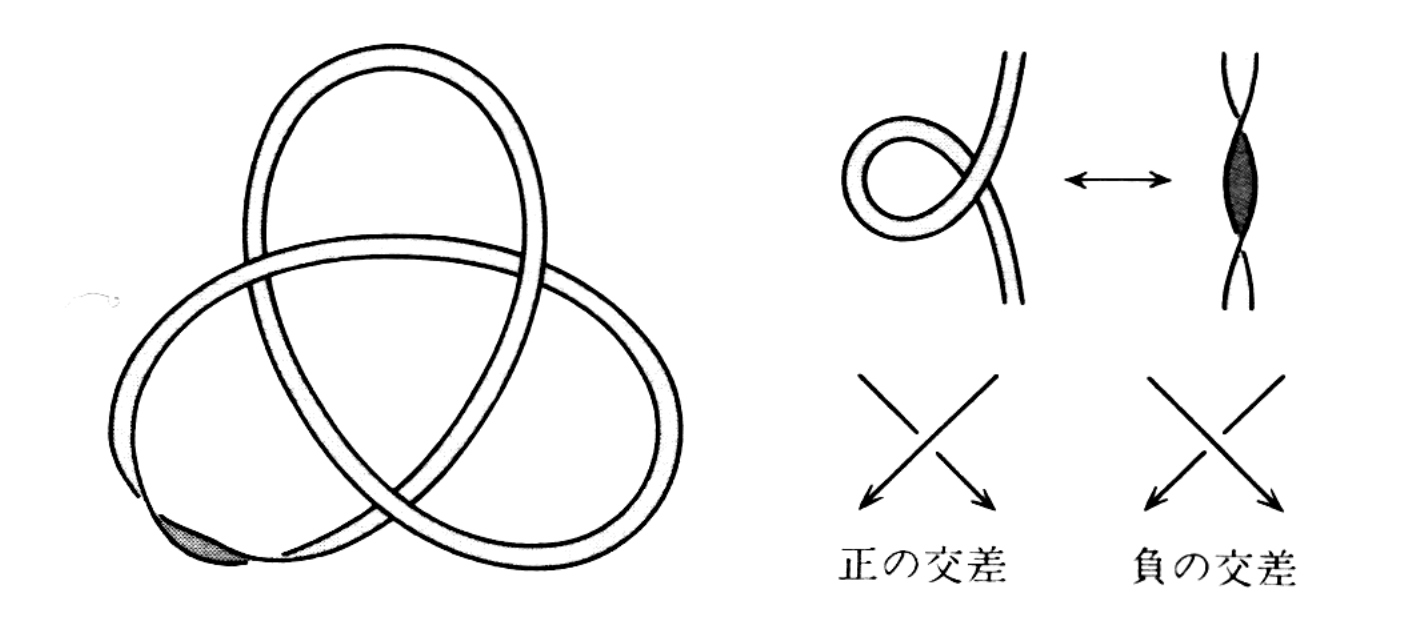
\includegraphics[width=0.94\textwidth]{figures/fig2.7.png}
  \figtitle{2.7}{framing 的带状表示。左图是对称为 trefoil 的纽结赋予 framing $4$ 的图示（原书 p.64）}
\end{figure}

% [Tutor Note: 图 2.7 中正负交叉的约定依赖两条分支的定向：把其中一条分支的定向反转，同一交叉便由正变负。$S^3$ 中链环的环绕数必须先固定各分支定向才有定义。]

设 $L$ 是 $\R^3$ 中带定向与 framing 的链环。首先，把仿射 Lie 代数 $\hat{\fg}$ 的 level $k$ 的最高权 $\lambda_1,\dots,\lambda_m$ 分别对应到链环的分支 $L_1,\dots,L_m$ 上。把链环的投影图取在 $xt$ 平面上 $x>0$ 的部分，如图 2.8 那样使极大点、极小点全部孤立，且极大值、极小值全部互不相同。再用直线 $t=t_j$（$j=0,1,2,\dots,s$）切开该图，使 $t_j<t<t_{j+1}$ 的部分是辫群生成元 $\sigma_i$ 对应的图、$\sigma_i^{-1}$ 对应的图，或只含一个极大点或极小点的图
% [原文 p.65]
中的一种。这四种图称为基本 tangle（elementary tangle）。不过，基本 tangle 中出现的曲线定向须考虑全部可能情形。特别地，约定直线 $t=t_0$、$t=t_s$ 与链环图不相交。设直线 $t=t_j$ 与链环图的交点为 $q_1,\dots,q_n$，按下述规则给各点配最高权：若过点 $q_j$ 的链环分支带有最高权 $\lambda$，则当链环的定向在 $q_j$ 处向下时配 $\lambda$，向上时配 $\lambda^\ast$。再给原点 $O$ 与无穷远点 $\infty$ 各配最高权 $0$，并用引理 1.13 的限制映射 $i^\ast$ 把相应的共形块空间嵌入不变张量空间。这样，与 $t_j$ 对应所得的线性空间记为 $V(t_j)$。特别地，$V(t_0)=V(t_s)=\C$。

\begin{figure}[htbp]
  \centering
  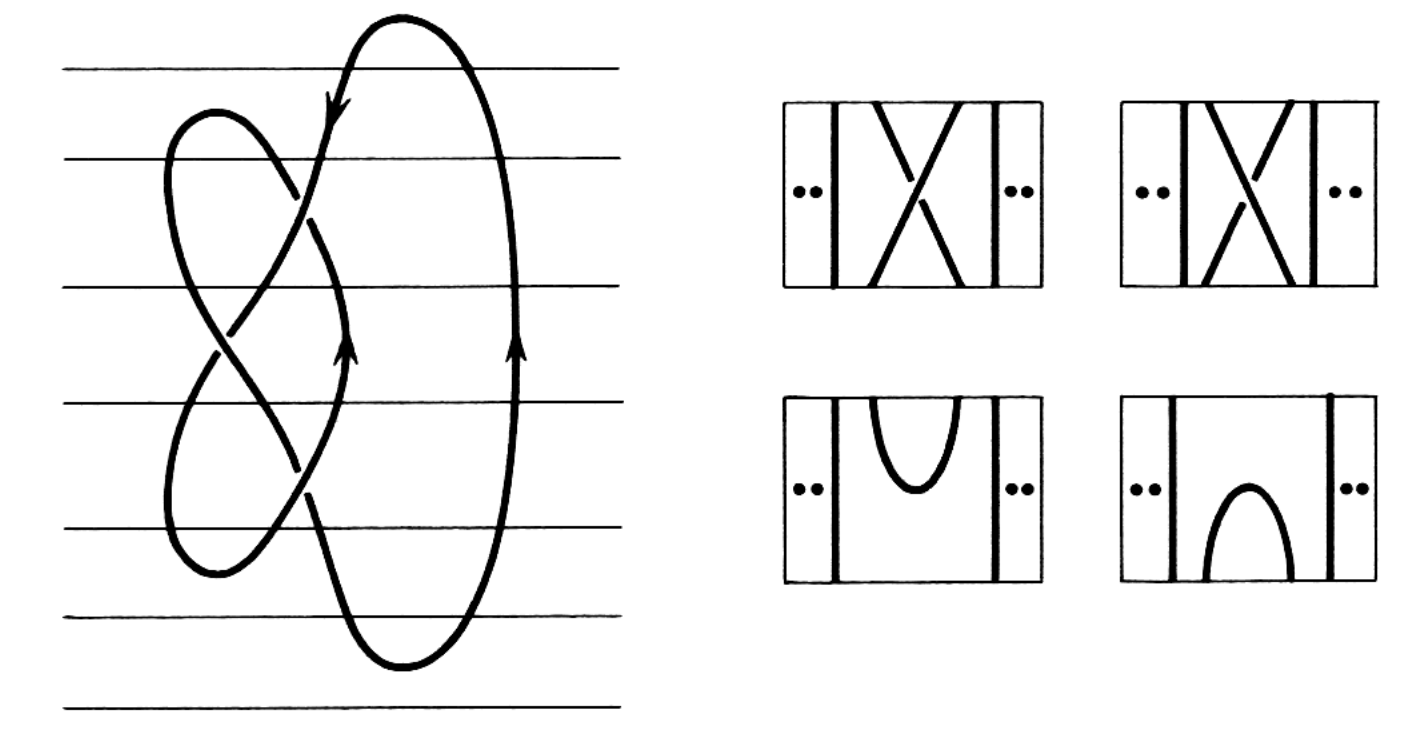
\includegraphics[width=0.94\textwidth]{figures/fig2.8.png}
  \figtitle{2.8}{把链环的图横着切开，分解为右图中的基本 tangle（原书 p.65）}
\end{figure}

对应于图 2.8 的基本 tangle，可以定义线性映射
\begin{equation}
  Z_j: V(t_j) \longrightarrow V(t_{j+1}),\qquad 0\le j\le s-1 \tag{2.24}
\end{equation}
具体说来，对辫群元素 $\sigma_i,\sigma_i^{-1}$ 对应的图，可由前节所述的 KZ 方程的单值表示定出线性映射；对极大点、极小点，则如图 2.9 那样补上最高权 $0$ 的表示，用前节讨论的 KZ 方程的连接矩阵定出线性映射。

% [原文 p.66]
\begin{figure}[htbp]
  \centering
  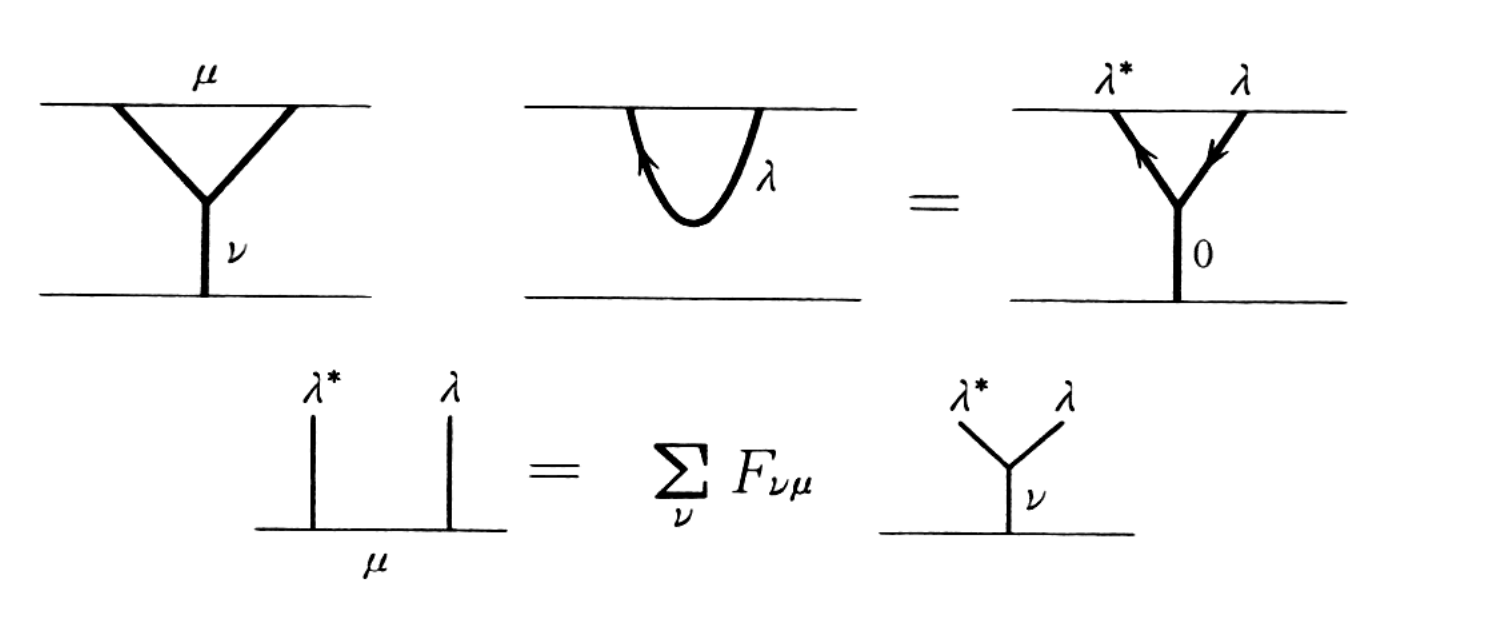
\includegraphics[width=0.96\textwidth]{figures/fig2.9.png}
  \figtitle{2.9}{极小点与 KZ 方程的连接矩阵（原书 p.66）}
\end{figure}

把线性映射 $Z_j$（$0\le j\le s-1$）依次合成，置
\begin{equation}
  Z(L;\lambda_1,\dots,\lambda_m)=Z_{s-1}\circ\cdots\circ Z_1\circ Z_0(1) \tag{2.25}
\end{equation}
由 KZ 连接的平坦性得到下述引理。

\begin{lemma}{2.4}
  $Z(L;\lambda_1,\dots,\lambda_m)$ 在图 2.10 所示的链环水平方向局部变形下不变。
\end{lemma}

\begin{figure}[htbp]
  \centering
  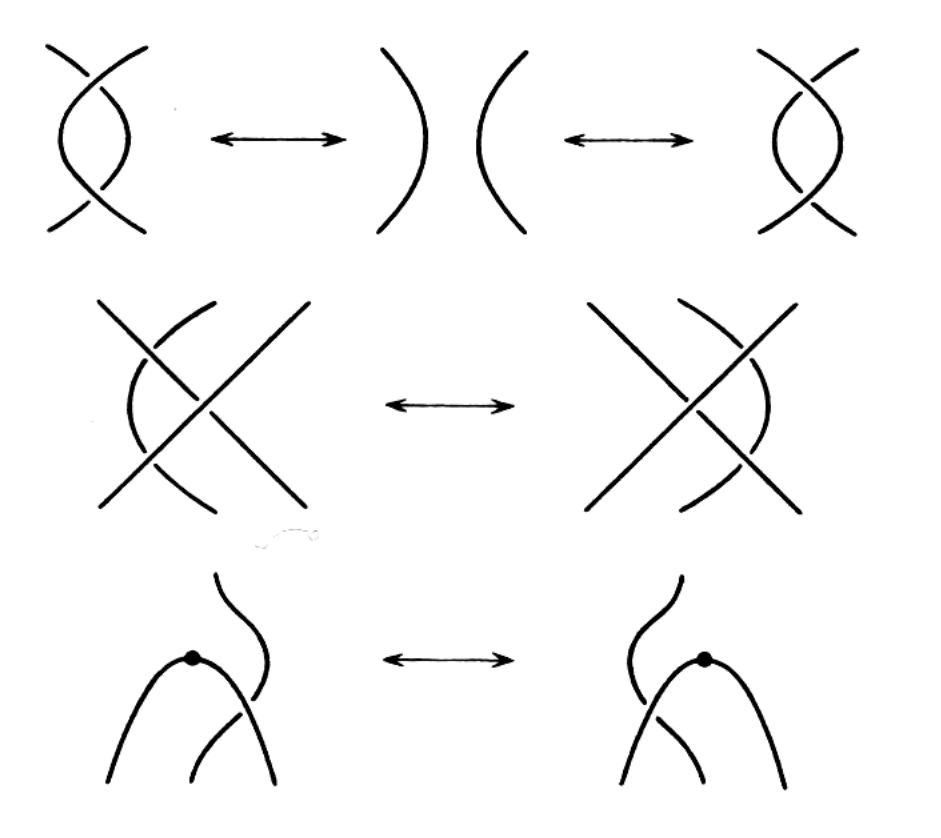
\includegraphics[width=0.55\textwidth]{figures/fig2.10.png}
  \figtitle{2.10}{链环水平方向的局部变形（原书 p.66）}
\end{figure}

% [Tutor Note: 图 2.10 的三种变形分别对应辫关系 $\sigma_i\sigma_{i+1}\sigma_i=\sigma_{i+1}\sigma_i\sigma_{i+1}$、互不相邻生成元的交换，以及极大点与极小点沿曲线的移动；引理的实质就是 KZ 连接的平坦性。]

$Z(L;\lambda_1,\dots,\lambda_m)$ 对图 2.11 所示两个临界点的对消操作并不具有不变性，因此下面作如下修正。把图 2.11 右端画出的、各有 $2$ 个极大点与 $2$ 个极小点、framing 为 $0$ 的平凡纽结记为 $K_0$，置
\[
  d(\lambda)=Z(K_0;\lambda)^{-1}.
\]
% [原文 p.67]
并置
\[
  J(L;\lambda_1,\dots,\lambda_m)=d(\lambda_1)^{\mu_1}\cdots d(\lambda_m)^{\mu_m}Z(L;\lambda_1,\dots,\lambda_m),
\]
其中 $\mu_j$ 表示链环分支 $L_j$（$1\le j\le m$）的极大点个数。

% [Tutor Note: 归一化所用的是极大点个数 $\mu_j$，而不是「极大点个数减极小点个数」。任何链环分支的投影图上极大点与极小点成对出现、个数相等，故两种计数给出的幂次相同；若把图 2.11 的约定改成以极小点归一，$d(\lambda)$ 的幂次会整体变号。]

\begin{figure}[htbp]
  \centering
  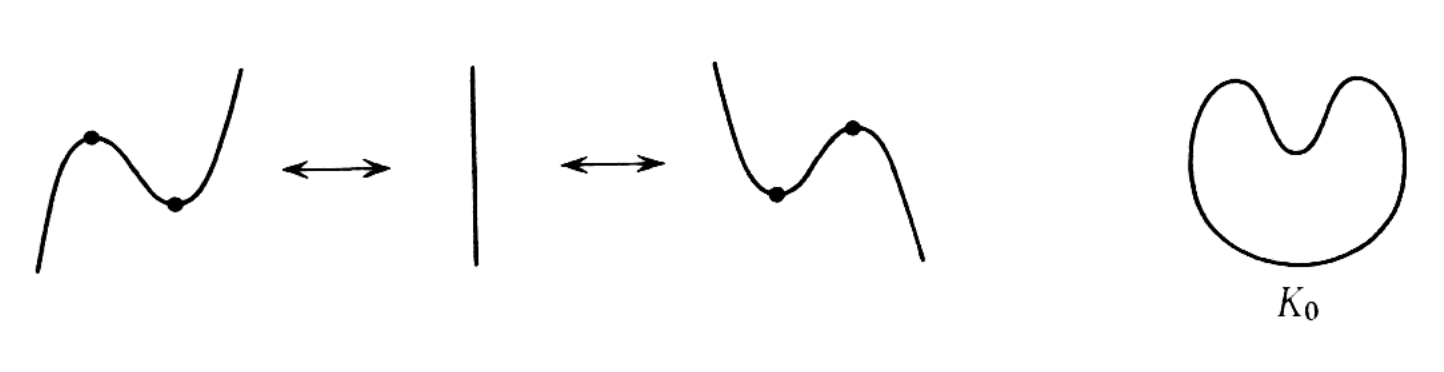
\includegraphics[width=0.94\textwidth]{figures/fig2.11.png}
  \figtitle{2.11}{左图为两个临界点的对消操作（原书 p.67）}
\end{figure}

这里约定链环各分支已编号；在链环等价的定义中，只考虑保持分支编号的同胚。已知在这个意义下，链环等价当且仅当二者能通过图 2.10、2.11 所示的局部变形互相迁移，于是得到下述定理。

\begin{theorem}{2.5}
  $J(L;\lambda_1,\dots,\lambda_m)$ 是给定各分支定向与 framing、并给定分支编号的链环的拓扑不变量。
\end{theorem}

由定理 2.3 之后说明的 $M_{0,n}$ 的作用，可得关于 framing 变化的下一命题。

\begin{proposition}{2.6}
  设 $L'$ 是把链环 $L=\bigcup_{j=1}^{m}L_j$ 的分支 $L_j$ 的 framing 增加 $1$ 所得的链环，则
  \[
    J(L';\lambda_1,\dots,\lambda_m)=\exp(2\pi\sqrt{-1}\Delta_{\lambda_j})\,J(L;\lambda_1,\dots,\lambda_m)
  \]
  成立。
\end{proposition}

特别地，当 $\lambda=1$ 时，给链环的每个分支都配 $\lambda$，考虑 $J(L;\lambda,\dots,\lambda)$

\begin{figure}[htbp]
  \centering
  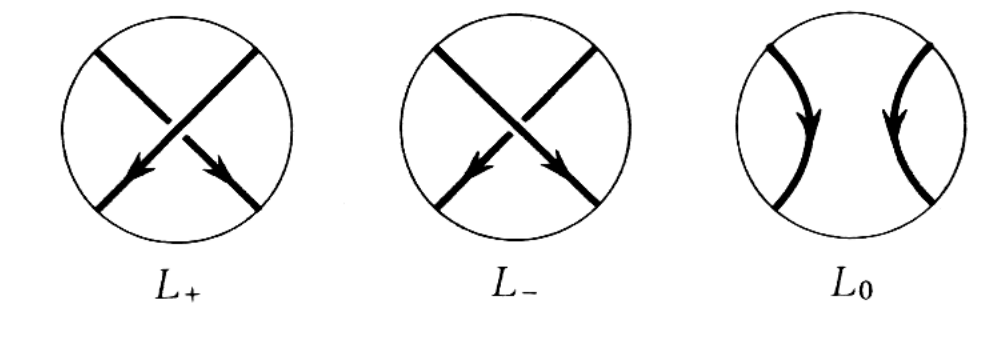
\includegraphics[width=0.62\textwidth]{figures/fig2.12.png}
  \figtitle{2.12}{原书无图注（原书 p.67）}
\end{figure}

% [Tutor Note: 图 2.12 的三幅图给出 $L_+$、$L_-$、$L_0$ 的局部替换：圆内分别是正交叉、负交叉与两条不相交的弧，圆外部分完全固定。拆接关系式比较的正是这三者在同一位置的不同。]

% [原文 p.68]
并记为 $J_L$。把链环图作如图 2.12 的局部变形所得的链环分别记为 $L_+,L_-,L_0$。这些不变量 $J_{L_+},J_{L_-},J_{L_0}$ 之间总存在称为拆接关系式（skein relation）的关系，下面叙述。$J_L$ 的拆接关系式如下：置
\[
  q^{1/m}=\exp\frac{2\pi\sqrt{-1}}{m(k+2)},
\]
这时下述命题成立。

\begin{proposition*}{2.7}
  $J_L$ 满足拆接关系式
  \[
    q^{1/4}J_{L_+}-q^{-1/4}J_{L_-}=(q^{1/2}-q^{-1/2})J_{L_0}.
  \]
\end{proposition*}

\begin{proof}
  §2.1 给出的辫子 $\sigma_i$ 的表示矩阵 $G_i=\rho(\sigma_i)$，如定理 2.3 的证明中所述，满足最小多项式
  \[
    (G_i+q^{-3/4})(G_i-q^{1/4})=0.
  \]
  将此式变形得
  \[
    q^{1/4}G_i-q^{-1/4}G_i^{-1}=(q^{1/2}-q^{-1/2})\,\mathrm{id}.
  \]
  按定义，$J_L$ 表为基本 tangle 对应线性映射的合成。比较 $L_+,L_-,L_0$ 用基本 tangle 合成的表示，可见只有一处不同：分别为正辫子 $\sigma_i$、负辫子 $\sigma_i^{-1}$ 与平凡辫子，其余基本 tangle 都一致。因此由 $G_i$ 满足的上述关系式，立即得到 $J_L$ 的拆接关系式。
\end{proof}

% [Tutor Note: 此处的 $q$ 与 §2.1 的 $q$ 差一个 $m$ 次根：$q^{1/m}=\exp(2\pi\sqrt{-1}/(m(k+2)))$。拆接关系式含 $q^{\pm1/4}$、$q^{\pm1/2}$，故必须先固定 $q^{1/m}$ 的分支；$q$ 为单位根这一事实使 $J_L$ 良定义，也使它化为 Jones 多项式的特殊值。]

拆接关系式可以从共形块空间的角度理解如下。
% [原文 p.69]
如图 2.13 把情形局部化，考虑 Riemann 球面上 $4$ 个点分别指定最高权 $\lambda_1,\lambda_2,\lambda_3,\lambda_4$ 的共形块空间。此时它们可用 $sl_2(\C)$ 的二维不可约表示的最高权 $\lambda$ 写成 $\lambda,\lambda,\lambda^\ast,\lambda^\ast$，故由命题 1.15 知共形块空间是 $2$ 维的。对应于 tangle $L_+,L_-,L_0$ 得到共形块空间之间的线性映射；共形块空间既为 $2$ 维，这 $3$ 个线性映射之间就有一个一次关系式。把它具体写出，正是上面的拆接关系式。

% [Tutor Note: $2$ 维共形块空间中的三个线性映射必线性相关，这就是拆接关系式的来源；系数 $q^{\pm1/4}$、$q^{\pm1/2}$ 由命题 1.15 的融合规则（即 $F$ 矩阵）唯一确定，并非任意选取。]

\begin{figure}[htbp]
  \centering
  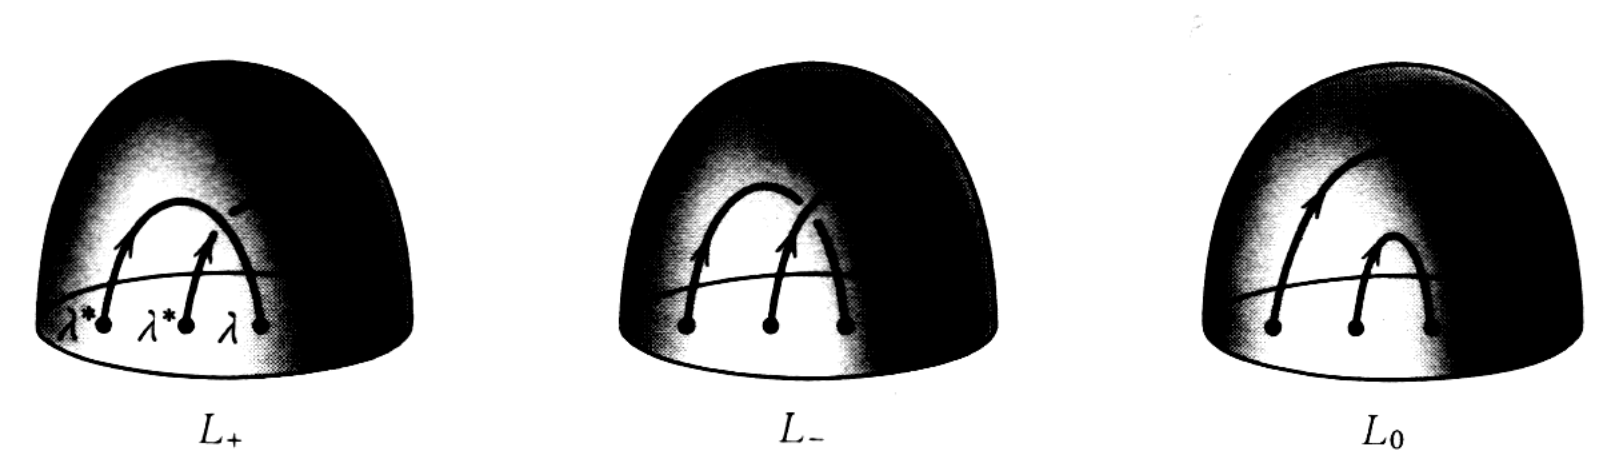
\includegraphics[width=0.96\textwidth]{figures/fig2.13.png}
  \figtitle{2.13}{共形块与拆接关系式（原书 p.69）}
\end{figure}

所构造的链环不变量 $J_L$ 依赖于链环 framing 的指定。为构造不依赖 framing 的不变量，在链环 $L$ 的图中，把正交叉个数减去负交叉个数记为 $w(L)$，置
\[
  P_L=d(1)^{-1}\exp\bigl(-2\pi\sqrt{-1}\,\Delta_1\,w(L)\bigr)J_L.
\]
由命题 2.6 可知，$P_L$ 是不依赖 framing 的、带定向链环的不变量。再比较 $w(L_+),w(L_-),w(L_0)$ 并用命题 2.7，可知 $P_L$ 满足拆接关系式
\[
  qP_{L_+}-q^{-1}P_{L_-}=(q^{1/2}-q^{-1/2})P_{L_0},
\]
且对平凡纽结有
\[
  P_{\bigcirc}=1.
\]
这是 Jones 多项式的一个版本。Jones 多项式是由拆接关系式
\[
  t^{-1}V_{L_+}-tV_{L_-}=(t^{1/2}-t^{-1/2})V_{L_0},\qquad V_{\bigcirc}=1
\]
刻画的链环不变量，取值于 Laurent 多项式环 $\Z[t^{1/2},t^{-1/2}]$。这里得到的 $P_L$，就是在 Jones 多项式中把变量 $t^{1/2}$ 换成 $-q^{-1/2}$ 所得。这样由共形场理论导出的 Jones 多项式在单位根处的特殊值，在下一节说明的三维流形 Witten 不变量的构造中起重要作用。若想从共形场理论的立场得到以 $t$ 为变量的原形 Jones 多项式，只需在以上讨论中把 $k$ 当作一般参数，并把 $\cH_{k,\lambda}$ 换成 Verma 模 $M_{k,\lambda}$
% [原文 p.70]
再按上述构造进行即可。

先把构造不变量时作为正规化常数引入的 $d(\lambda)$ 在 $\lambda=1$ 时算出来。当 $L_+,L_-,L_0$ 取图 2.14 的三个链环时，$P_{L_+}=1$、$P_{L_-}=1$、$P_{L_0}=d(1)$，于是用拆接关系式可知
\[
  d(1)=\frac{q-q^{-1}}{q^{1/2}-q^{-1/2}}.
\]

\begin{figure}[htbp]
  \centering
  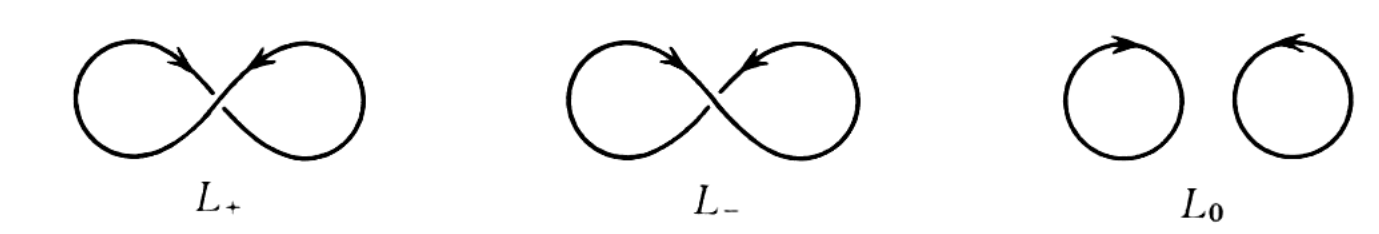
\includegraphics[width=0.85\textwidth]{figures/fig2.14.png}
  \figtitle{2.14}{由拆接关系式计算 $d(1)$（原书 p.70）}
\end{figure}

% [Tutor Note: 图 2.14 的 $L_0$ 是两个互不相交的平凡纽结，其不变量并不等于 $d(1)$ 本身：由命题 2.10，两分支权皆为 $1$ 时 $J_{L_0}=d(1)^2$，而 $P_L$ 还含因子 $d(1)^{-1}$，故 $P_{L_0}=d(1)$。原书略去了这一步。]

直到现在，我们看到的是给各分支最高权 $1$ 时的不变量，它基本上是 Jones 多项式的特殊值。一般地，给各分支 level $k$ 的最高权 $\lambda_1,\dots,\lambda_m$ 时，可以如下由称为 cabling 的操作与 §1.6 说明的融合代数 $R_k$ 的结构计算不变量 $J(L;\lambda_1,\dots,\lambda_m)$。对给定 framing $t$ 的纽结 $K=K_0$，如图 2.15 那样，在 $K_0$ 的管状邻域边界上重新给定纽结 $K_1$，使它与 $K_0$ 的环绕数等于 $t$
% [原文 p.71]
的操作称为 cabling。$K_1$ 也赋予 framing $t$。这样得到有两个分支的链环 $K_0\cup K_1$。

\begin{figure}[htbp]
  \centering
  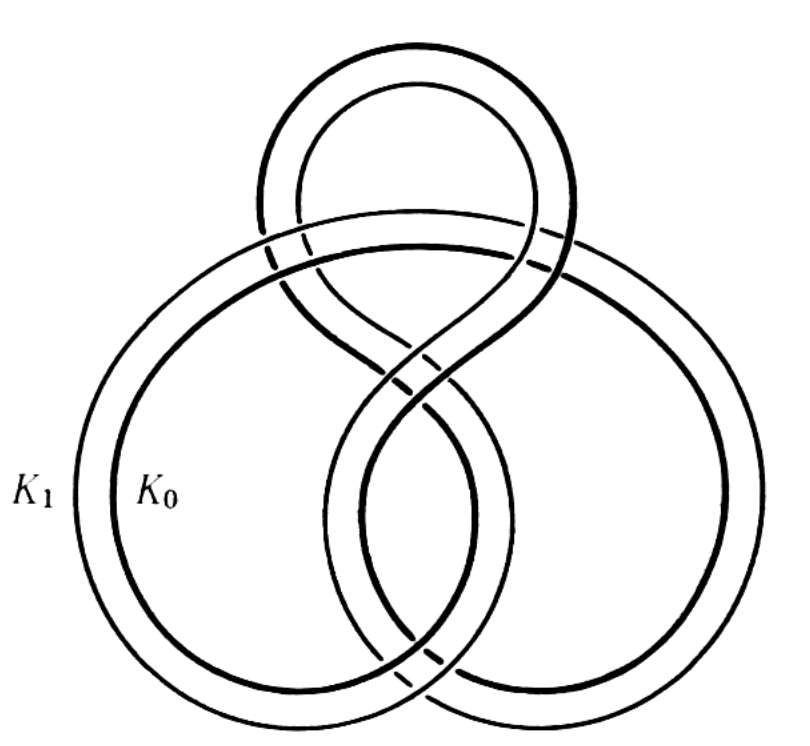
\includegraphics[width=0.42\textwidth]{figures/fig2.15.png}
  \figtitle{2.15}{纽结 $K_0$ 的 cabling（原书 p.70）}
\end{figure}

\begin{lemma}{2.8}
  当给上述 cabling 操作所得链环 $K_0\cup K_1$ 的各个分支分别赋予 level $k$ 的最高权 $\lambda,\mu$ 时，
  \[
    J(K_0,K_1;\lambda,\mu)=\sum_{\nu}N_{\lambda\mu}^{\nu}J(K;\nu)
  \]
  成立。这里 $N_{\lambda\mu}^{\nu}$ 是融合代数 $R_k$ 的结构常数。
\end{lemma}

% [Tutor Note: 原书此式右端写作 $J(K;\nu)$，而 $K$ 在前文并未定义（cabling 的两个分支记作 $K_0,K_1$）。按上下文与引理 2.9 的用法，$K$ 应理解为本来的结 $K_0$；此处照原书抄录，未擅改。]

由上述引理，可以给链环的各分支配上融合代数 $R_k$ 的元素 $x_1,\dots,x_m$，从而定义不变量 $J(L;x_1,\dots,x_m)$。首先，当 $x_1,\dots,x_m$ 是最高权 $\lambda_1,\dots,\lambda_m$ 对应的元素时，照旧定义为 $J(L;\lambda_1,\dots,\lambda_m)$。接下来把它归纳地扩充到融合代数 $R_k$ 上：当给某个分支 $L_j$ 配上积 $v_\lambda\cdot v_\mu\in R_k$ 时，对 $L_j$ 施行上述 cabling 操作，给所得各分支分别配 $\lambda,\mu$ 来定义。由引理 2.8，它可以表为原链环 $L$ 的不变量的线性组合。这样，多重线性映射
\[
  J(L): R_k^{\otimes m}\longrightarrow \C
\]
便由 $J(L)(x_1,\dots,x_m)=J(L;x_1,\dots,x_m)$ 确定。一般地，$J(L;\lambda_1,\dots,\lambda_m)$ 的计算可通过 cabling 操作增加链环分支的个数，归结为给所有分支都配最高权 $1$ 的链环的不变量的计算。

再列举不变量 $J(L;\lambda_1,\dots,\lambda_m)$ 的其他性质。

\begin{lemma*}{2.9}
  设 $K$ 为平凡纽结，给它 framing $0$ 与 level $k$ 的最高权 $\lambda$。此时
  \[
    J(K;\lambda)=d(\lambda)=\frac{q^{(\lambda+1)/2}-q^{-(\lambda+1)/2}}{q^{1/2}-q^{-1/2}}
  \]
  成立。
\end{lemma*}

\begin{proof}
  首先注意，用式 (1.42) 的 $S_{\lambda\mu}$ 可写
  \[
    \frac{q^{(\lambda+1)/2}-q^{-(\lambda+1)/2}}{q^{1/2}-q^{-1/2}}=\frac{S_{0\lambda}}{S_{00}}.
  \]
% [原文 p.72]
  又，取 $K$ 为赋予 framing $0$ 的平凡纽结时，由 $J(K;\lambda)$ 的定义，$J(K;\lambda)=d(\lambda)$ 立即成立。对平凡纽结作 cabling，可知
  \begin{equation}
    d(\lambda)d(\mu)=\sum_{\nu}N_{\lambda\mu}^{\nu}d(\nu) \tag{2.26}
  \end{equation}
  成立。此外，$d(\lambda)$ 由式 (2.26) 与 $d(1)$ 的值刻画。$d(1)$ 已经给出，故只需证明 $d(\lambda)=S_{0\lambda}/S_{00}$ 确实满足式 (2.26)。这可用命题 1.22 所示的 Verlinde 等式加以确认。
\end{proof}

% [Tutor Note: 这里 $d(\lambda)$ 有两个来源：一处由 $J(K;\lambda)$ 定义，一处由 $S_{0\lambda}/S_{00}$ 给出。证明的思路是先验证后者满足式 (2.26)、再用「式 (2.26) 加 $d(1)$ 的值唯一确定 $d(\lambda)$」把两者接上；Verlinde 等式正是用来验证式 (2.26) 的。]

以下常把 $J(L;\lambda_1,\dots,\lambda_m)$ 简记为 $J(L;\lambda)$。对由两个链环 $L_1,L_2$ 的并集给出的链环 $L_1\cup L_2$，用最高权序列 $\mu_1$ 指定 $L_1$ 各分支的权、用最高权序列 $\mu_2$ 指定 $L_2$ 各分支的权，所得不变量记为 $J(L_1\cup L_2;\mu_1\cup\mu_2)$。下一命题可由不变量 $J(L;\lambda)$ 的构造法直接得到。

\begin{proposition}{2.10}
  对分别包含在互不相交的三维球体 $B_1,B_2$ 中的链环 $L_1,L_2$，
  \[
    J(L_1\cup L_2;\mu_1\cup\mu_2)=J(L_1;\mu_1)J(L_2;\mu_2)
  \]
  成立。
\end{proposition}

链环 $L$ 的镜像记为 $\bar L$。也就是说，$\bar L$ 是由反转 $S^3$ 定向的同胚作用在 $L$ 上所得的像。至于 framing，取镜像后符号相反。对链环的镜像，下一命题成立。

\begin{proposition*}{2.11}
  设带定向与 framing 的链环 $L$ 的镜像为 $\bar L$，则
  \[
    J(\bar L;\lambda)=\overline{J(L;\lambda)}
  \]
  成立。这里右端表示 $J(L;\lambda)$ 的复共轭。
\end{proposition*}

\begin{proof}
  用 cabling 操作，命题的证明可归结为所有分支所给最高权均为 $1$ 的情形。此时 $d(\lambda)$ 为实数，再由命题 2.7 所示的 $J_L$ 的拆接关系式，得 $J_{\bar L}(q)=J_L(q^{-1})$；又 $q$ 是单位根，由此得到所求结论。
\end{proof}

% [Tutor Note: $q$ 为单位根时 $q^{-1}=\bar q$，所以 $J_L(q^{-1})=\overline{J_L(q)}$；若 $q$ 不是单位根，这一步不成立。这正是本章只在 $q$ 为单位根（即 $k$ 为正整数）时讨论不变量的原因。]

% [原文 p.73]
Jones 多项式方面，同样由拆接关系式可知 $V_{\bar L}(t)=V_L(t^{-1})$ 成立。图 2.16 是用拆接关系式算出的 trefoil 纽结（trefoil）及其镜像的 Jones 多项式。

\begin{figure}[htbp]
  \centering
  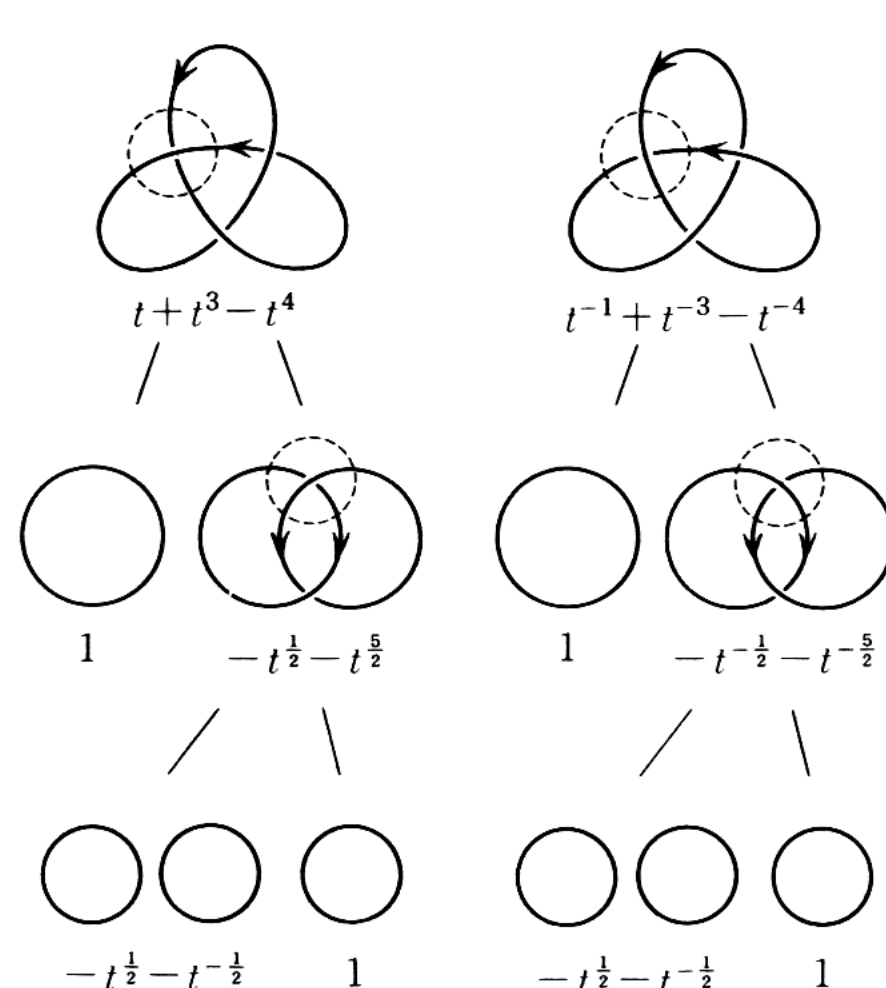
\includegraphics[width=0.60\textwidth]{figures/fig2.16.png}
  \figtitle{2.16}{trefoil 及其镜像的 Jones 多项式（原书 p.73）}
\end{figure}

% [Tutor Note: 图 2.16 中各值均为 Laurent 多项式：trefoil 为 $t+t^3-t^4$，把 $t$ 换成 $t^{-1}$ 得镜像的值 $t^{-1}+t^{-3}-t^{-4}$，正是本段所说的 $V_{\bar L}(t)=V_L(t^{-1})$。虚线圆标出每次作拆接的位置。]

对链环的上述构造可推广到带定向与 framing 的 tangle。先说明 tangle。取复平面 $\C$ 与单位区间 $[0,1]$ 的直积为 $X$。在 $X_0=\C\times\{0\}$ 内的实轴上取点 $p_1,\dots,p_m$，又在 $X_1=\C\times\{1\}$ 内的实轴上取点 $q_1,\dots,q_n$。$X$ 内以 $p_1,\dots,p_m,q_1,\dots,q_n$ 为边界的紧 $1$ 维流形，称为 $(m,n)$ tangle。tangle 用图 2.17 那样的投影图表示。tangle 的连通分支由若干闭曲线，以及以 $p_1,\dots,p_m,q_1,\dots,q_n$ 中某点为端点的弧组成。这里给所有这些连通分支都指定定向，并给各分支赋予 framing。

链环的不变量 $J(L;\lambda)$ 的构造方式是：给链环各分支配最高权，把链环横着切分、分解成基本 tangle，给各个 level 配上共形块空间，再把基本 tangle 对应
% [原文 p.74]
的共形块空间之间的线性映射合成起来。看这个过程可知，对上述 $(m,n)$ tangle，也可给 tangle 的各个连通分支配最高权，从而构造从 $X_0$ 对应的共形块空间到 $X_1$ 对应的共形块空间的线性映射。

把这个构造再具体说明一下。首先，对以 $p_1,\dots,p_m,q_1,\dots,q_n$ 中某点为端点的弧，指定 level $k$ 的最高权。对每个点 $p_1,\dots,p_m,q_1,\dots,q_n$，若过该点的弧向下，则对应到该弧所配的表示；若过该点的弧向上，则对应到该表示的对偶表示。这样，设配给 $p_1,\dots,p_m$ 的表示的最高权为 $\mu_1,\dots,\mu_m$，配给 $q_1,\dots,q_n$ 的表示的最高权为 $\nu_1,\dots,\nu_n$。再给 $(m,n)$ tangle $T$ 中由闭曲线构成的各连通分支配 level $k$ 的最高权，记作 $\lambda$。把 $(m,n)$ tangle 分解为基本 tangle 的合成，便得到线性映射
\begin{equation}
  J(T;\lambda): V_{\mu_1\cdots\mu_m}\longrightarrow V_{\nu_1\cdots\nu_n}, \tag{2.27}
\end{equation}
称之为 tangle 算子（tangle operator）。

下一命题也可立即得到。

\begin{proposition}{2.12}
  把带定向与 framing 的 $(1,1)$ tangle $T$ 闭合所得链环记为 $\hat T$。如图 2.17 给出权时，
  \[
    J(\widehat{T_1\circ T_2})=J(\hat T_1)J(\hat T_2)\,\frac{S_{00}}{S_{0\lambda}}
  \]
  成立。
\end{proposition}

% [Tutor Note: $\widehat{T_1\circ T_2}$ 的帽子覆盖整个合成 $T_1\circ T_2$，表示把合成后的 tangle 整体闭合；$\hat T_1,\hat T_2$ 则是分别闭合。两者是不同的链环，右端把两个闭合结果的不变量相乘，因子 $S_{00}/S_{0\lambda}$ 来自闭合处权 $\lambda$ 的收缩。]

用 tangle 算子还可以如下解释链环的不变量 $J(L;\lambda)$。如图 2.18 那样，用不经过极大点、极小点的水平平面切链环，把对应于该切口的共形块空间记为 $V(t)$。该平面下方的 tangle 记为 $T_+$，上方的 tangle 记为 $T_-$。由 $T_+$ 对应的 tangle 算子，$1$ 的像记为 $J(T_+)\in V(t)$。对 $T_-$ 则上下翻转，作同样的构造，
% [原文 p.75]
便定出 $J(T_-)\in V(t)^\ast$。用 $V(t)$ 与对偶空间 $V(t)^\ast$ 的自然配对，可以把 $J(L)$ 表为
\[
  J(L)=\langle J(T_+),J(T_-)\rangle.
\]
这种想法稍后将从拓扑场论的角度重新说明。

\begin{figure}[htbp]
  \centering
  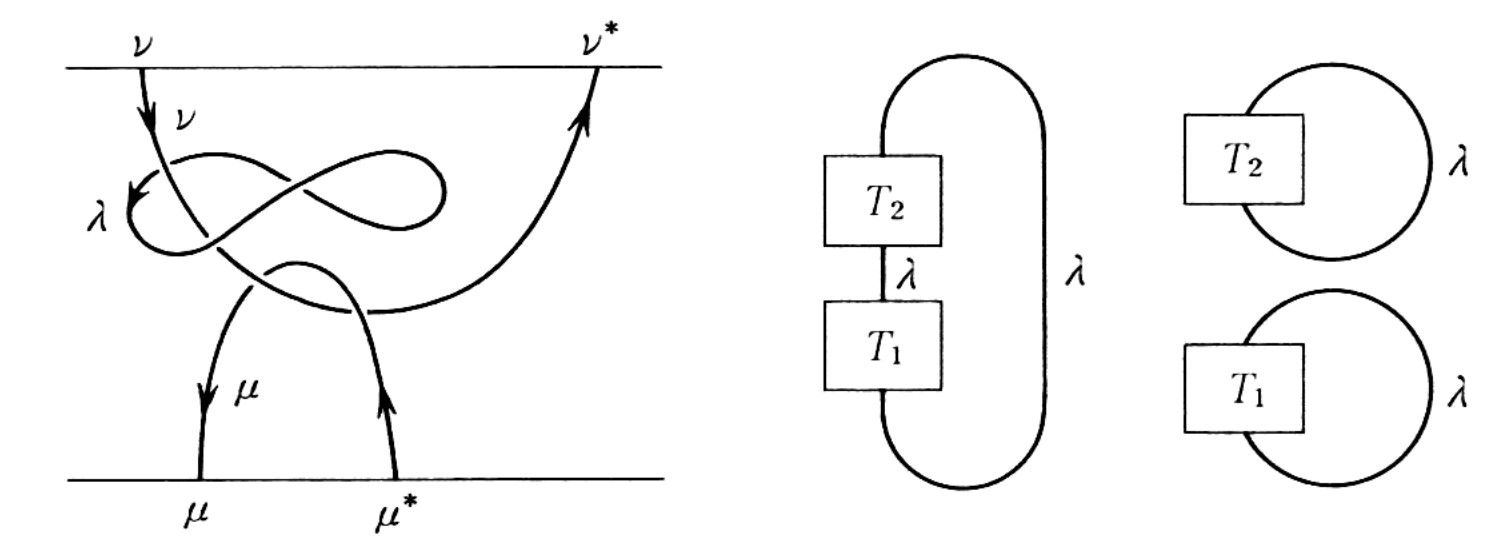
\includegraphics[width=0.96\textwidth]{figures/fig2.17.png}
  \figtitle{2.17}{原书无图注（原书 p.75）}
\end{figure}

\begin{figure}[htbp]
  \centering
  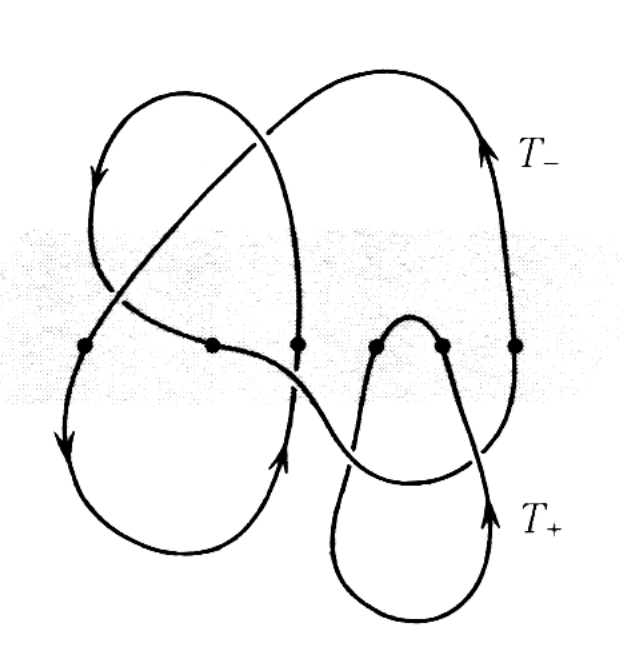
\includegraphics[width=0.36\textwidth]{figures/fig2.18.png}
  \figtitle{2.18}{原书无图注（原书 p.75）}
\end{figure}

% [Tutor Note: 对 $T_+$ 只看「$1$ 的像」，是因为 $T_+$ 的 tangle 算子是 $\C=V(t_0)\to V(t)$ 的映射；$T_-$ 上下翻转后其算子是 $V(t)\to\C$，故 $J(T_-)$ 落在对偶空间 $V(t)^\ast$ 中，与 $J(T_+)$ 配对即得标量 $J(L)$。]

\section{三维流形的 Witten 不变量}

\takeaway{以 $S^3$ 中带 framing 链环的 Dehn 手术表示任意闭可定向三维流形，再用共形场理论给出的链环不变量在 Kirby 操作下的不变性，定义三维流形的 Witten 不变量。}

本节用共形场理论，把 Witten 在论文 [1] 中从 Chern--Simons 规范理论的角度提出的三维流形拓扑不变量加以定式化。

设 $L$ 是 $S^3$ 内的、带 framing 的链环。对这种 $L$，通过下面说明的称为 Dehn 手术的操作，可以构造三维
% [原文 p.76]
流形。设 $L$ 的分支为 $L_1\cup\cdots\cup L_m$，取 $L$ 的管状邻域 $N(L)=N(L_1)\cup\cdots\cup N(L_m)$。各个 $N(L_j)$（$1\le j\le m$）同胚于实心环面，即 $S^1$ 与二维圆盘 $D$ 的直积。在 $N(L_j)$ 的边界 $\partial N(L_j)$ 上指定一条给出纽结 $L_j$ 的 framing 的闭曲线 $\gamma_j$。$\gamma_j$ 与 $L_j$ 的环绕数就是确定 $L_j$ 的 framing 的整数。又取 $H_j\cong D\times S^1$（$1\le j\le m$）为实心环面的 $m$ 个副本，在各自边界上给定经线（meridian）$m_j$。所谓经线，是固定 $S^1$ 上的点 $p$ 后表为 $\partial D\times\{p\}$ 的、$\partial H_j$ 上的闭曲线。置 $E(L)=S^3\setminus N(L)$。$E(L)$ 的边界表为
\[
  \partial E(L)=\partial N(L_1)\cup\cdots\cup\partial N(L_m).
\]
其次，取同胚
\[
  f:\partial H_1\cup\cdots\cup\partial H_m\longrightarrow \partial N(L_1)\cup\cdots\cup\partial N(L_m),
\]
使之满足 $f(m_j)=\gamma_j$（$1\le j\le m$）。用同胚 $f$ 把 $E(L)$ 与 $H_1\cup\cdots\cup H_m$ 沿边界粘合所得的三维流形记为 $M_L$。这样，挖去链环 $L$ 的管状邻域、再依照 framing 把实心环面填回的这步操作，称为沿 $L$ 的 Dehn 手术（Dehn surgery）。$M_L$ 由带给定 framing 的链环 $L$ 的等价类、在相差同胚的意义下唯一确定。又已知：所有带定向、无边界紧三维流形，都能由沿某个带 framing 链环 $L$ 的 Dehn 手术得到。

$M_L$ 还可以如下表为四维流形的边界。首先取以 $S^3$ 为边界的四维球体 $B^4$，在 $B^4$ 上依 $L\subset\partial B^4$ 的 framing 粘上 $2$-柄所得的四维流形记为 $W_L$，则 $M_L=\partial W_L$。下面给 Dehn 手术一个简单例子。设 $K$ 为平凡纽结。给 $K$ 赋予 framing $1$ 作 Dehn 手术，所得流形是 $S^3$。又，给平凡纽结 $K$ 赋予 framing $0$ 作 Dehn 手术，得到 $S^2\times S^1$。

% [Tutor Note: $E(L)=S^3\setminus N(L)$ 是链环的外部，其边界是 $m$ 个环面；$f$ 把实心环面的经线送到 framing 曲线 $\gamma_j$。因此这里的「framing」并不是额外的装饰，它等价于粘合映射 $f$ 的选取。]

% [Tutor Note: 平凡纽结作 framing $n$ 的 Dehn 手术得透镜空间 $L(n,1)$：$n=\pm1$ 时为 $S^3$，$n=0$ 时为 $S^2\times S^1$。可见同一三维流形可由不同的链环得到，这正是下一节引入 Kirby 操作的缘由。]

% [Tutor Note: $L\subset\partial B^4$ 的 framing 决定 $2$-柄的粘法；$W_L$ 的构造说明 Dehn 手术是四维柄分解的一部分，$M_L=\partial W_L$ 把三维流形的同胚问题化为链环的 Kirby 等价问题。]

% CHUNK ch02b DONE
